This chapter provides an overview for the development of problems in this project. The development of tools and problems is inspired by the methodology used in the book: \textit{"Knowledge Engineering Tools and Techniques for AI Planning"} by Mauro Vallati \cite{strobel_mypddl_2020}.

\section{Management}
\subsection{Methodology}
This project was developed with a centre focus around the generation of problems, so that the planner could achieve the best results from the problem. The development started with a \textit{problem generator} foundation that allowed for the development of new generators to be completed more efficiently and effectively without having to redefine the structure for each environment. After each problem generator was created, both classical and generalised plans were be synthesised from the problems generated, and measured to ensure that the algorithm employed within it were performing as expected. If it did not perform as expected, the changes would be re-designed with a new approach. This iterative development process led to robust algorithms that yield optimal results in experiments. Furthermore, this allowed the aims of this project to be worked towards more effectively. The description of these problem generators are described in the following sections.

\subsection{Chosen Language}
The chosen language for this project is Python. This has been chosen notably due to the library and community support with PDDL; and its popularity within the field of automated planning. Python allows for fast development due to its simple and understandable syntax \cite{druzhinina_why_2023}\cite{scarlett_why_2023}. Furthermore, Python has been covered extensively during teaching, which in turn has reduced the amount of time needed to learn the language. This is especially important given the time restrictions on this project.\\\\
Python is an object-oriented language, which is key in the design of the problem generators covered in the following sections. Python also contains a unique datatype \texttt{tuple}, which is an ordered, unchangeable and indexed collection. This is used for creating references to locations in an environment. For example, the position $(x, y)$ can be expressed directly in Python as a tuple \texttt{(x, y)}.

\subsubsection{Alternative choice of language}
Another language that was considered was C++ as both planners are developed in C++, and it is well known for its fast execution speeds and memory management tools.\cite{noauthor_why_2023} However, C++ lacks in PDDL library support, and the syntax is significantly more complex than Python, which would require investing a lot of time learning before being able to start working on the project itself.

\subsection{Libraries}
\subsubsection{Unified Planning}
For PDDL utility, the Unified Planning library was used, which contain a wide variety of PDDL tools. This is used mainly to bridge the gap between problem generators developed in Python and domains written in PDDL. The \texttt{PDDLReader} provides a parsing utility that allowed for PDDL problems to be created in Python, whilst referencing the domain in PDDL. Furthermore, Unified Planning contains a wide variety of planning engines that include Fast Downward and BFGP++. This reduced the time required to develop parsing tools and the complexity of having to run planners externally through bash scripts. 

\subsubsection{PyGame}
The visual aspects for environment generation is done through Pygame. There is an abundance of helpful resources and documentation. The reason for choosing this over more sophisticated tools such as OpenGL or Qt, is due to simplicity of designing images and that it is significantly more lightweight in comparison. It meets all the colouring and shape criteria required to create visuals for the path finding games described in the Background.

\section{Pipeline}
Figure 3.1 below shows the pipeline for the processing of a real world environment to a solution plan:

\begin{figure}[h!]
    \ctikzfig{images/pipeline}
    \caption{Design structure for Problem Generator}
\end{figure}

\noindent In the first stages of the pipeline, the agent's knowledge-base of the environment is represented within the domain, which as mentioned, contains the actions schema and predicates that correspond to what the agent can do within the environment. All the objects such as locations on the board, and information regarding the agents start and goal locations are processed within the problem generator. In the second stage, the problem generator observes the domain and produces a set of classical planning instances $\mathcal{P}$, which then can be processed by a planner. Finally, a classical planner observes each planning instance and produces a plan for each instance in $\mathcal{P}$. The generalised planner observes all planning instances at once and produces a single algorithm-like plan.

\section{Problem Generation}
This section covers the attributes that form part of a problem generator. All generators that inherit from this contain all these attributes along with additional functionality that is unique in each generator.

\subsection{Objects}
As described in the Background section of this report, an object represents a thing that forms part of an environment. To convert a real world object such as apples in the Snake game, it needs to be converted to a PDDL object. In this report, the function toObj$(x)$ converts an instance $x$ such as the position of an apple, and returns the PDDL object that it represents. To distinguish, the term \textit{environment object} refers to a real life object, and an \textit{object} refers to a PDDL object. Environment objects can also be positions, as they can be modelled in a PDDL object.

\subsection{Environments}
The abstraction of a domain in this project is an environment. An environment contains all representations of objects that will be used within a problem. Each environment has the structure
\begin{itemize}
    \item \textbf{Start}: An environment object representing a start state.
    \item \textbf{Setting}: A collection of environment objects that build up the setting that describes the environment, this could be a set of positions in which a player can traverse.
    \item \textbf{Goal}: An environment object representing the goal state, this could be the final location of the player.
\end{itemize}
There are two ways to create an environment in a problem generator:

\subsubsection{Manual Generation}
This form of generation allows the user to create their own environment for a domain in a Pygame window, the user can add environment objects through options set in the problem generator. The user is required to set a start and a goal state and it is not compulsory to set a winnable environment, allowing the user to create unsolvable problems as well as specific case problems that can't be achieved through automatic generation.

\subsubsection{Automatic Generation}
With automatic generation, the generator aims to randomly create winnable environments by greedily adding objects until there is one. This form of generation is typically used to rapidly generate problems for large scale experiments where manual generation is tedious.

\subsection{Tiles}
Positions on a board are represented by tiles. A tile is a mapping of an environment position in to the respective Pygame object. In the Pygame system, $(0, 0)$ is at the top-left most position on the display. When referring to a tile $t$ we always use its Pygame position. $t_x$ is the tiles $x$ position and $t_y$ is the $y$ position. Tiles are used widely in the generation of problems and hence locations in this report will be referred to as tiles. The number of tiles that can fit on a row on the display is given by $T$ hence the bottom-right most position on the display is $(T, T)$. This serves as the basis for scaling the size of problems within this report.

\subsubsection{Neighbouring Tiles}
As the agent can only move in 4 orientations, each tile can have a maximum of 4 neighbours. The possible neighbours of some tile $t$ are: $North: (t_x, t_y - 1)$, $East: (t_x - 1, t_y)$, 
$South: (t_x, t_y + 1)$ and $West: (t_x + 1, t_y)$. The function getNeighbours$(t)$ obtains all possible neighbours of the tile $t$ that are contained within the $T^2$ locations. Whereas $L.$findNeighbours$(t)$ obtains all possible neighbours that are contained within the array of tiles $L$. This is to ensure that tiles that do not belong within the environment are generated inside the PDDL problem or shown on the Pygame display.

\newpage
\section{Maze Problem Generation}
A Maze environment consists of three main components:

\begin{itemize}
    \item \textbf{Tiles}: A collection of tile objects representing the available locations for the player to traverse within the maze. The limit on the size of this collection is given by $T^2$  where $T$ is the maximum number of tiles displayable on a row on the display.
    \item \textbf{Start}: The initial location of the player $s_M$, there can only be one starting location per maze environment.
    \item \textbf{Goal}: The final destination of the player $g_M$, there can also only be one goal location per maze.
\end{itemize}

\subsection{Environment Generation}
\paragraph{Manual}
The environment can be generated manually through a Pygame interface. The user can select tiles on the screen to form part of the maze, marking it in yellow. Left-clicking a tile that is marked as being part of the maze will set the tile to either a start, marking the tile as red; or a goal tile, marking the tile as green. The start/goal tile selection is done in rotation, after a start tile has been selected, the next left-click on a tile will change it to a goal tile. The user is required to set a start and a goal state, however, it is not compulsory to set a winnable environment, allowing the user to create unsolvable problems as well as specific case problems that can't be achieved through automatic generation.

\begin{figure}[h!]
\centering
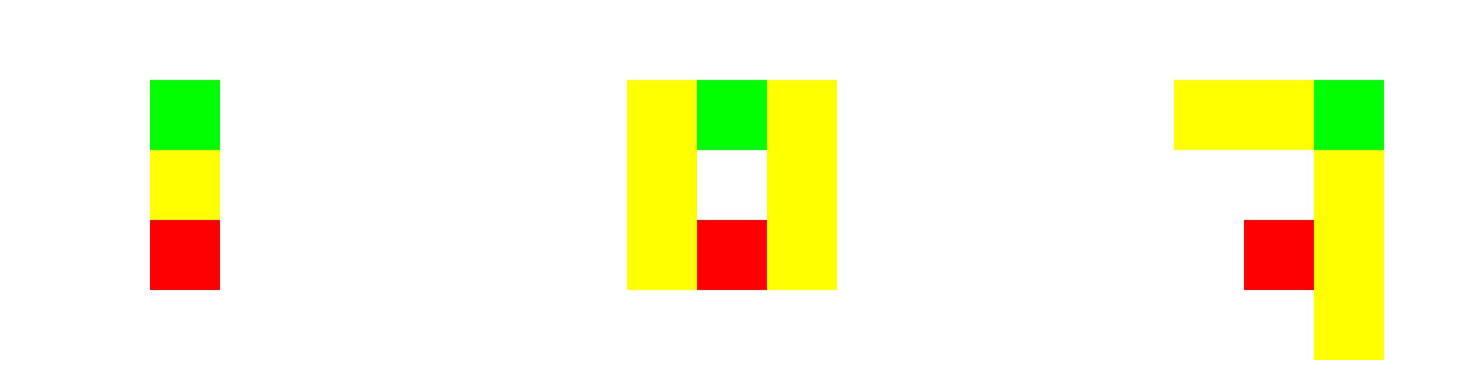
\includegraphics[width=\textwidth]{images/manual_maze_gen.png}
\caption{Examples of manually generated mazes ($T=5$)}
\end{figure}

\begin{figure}[h!]
\centering
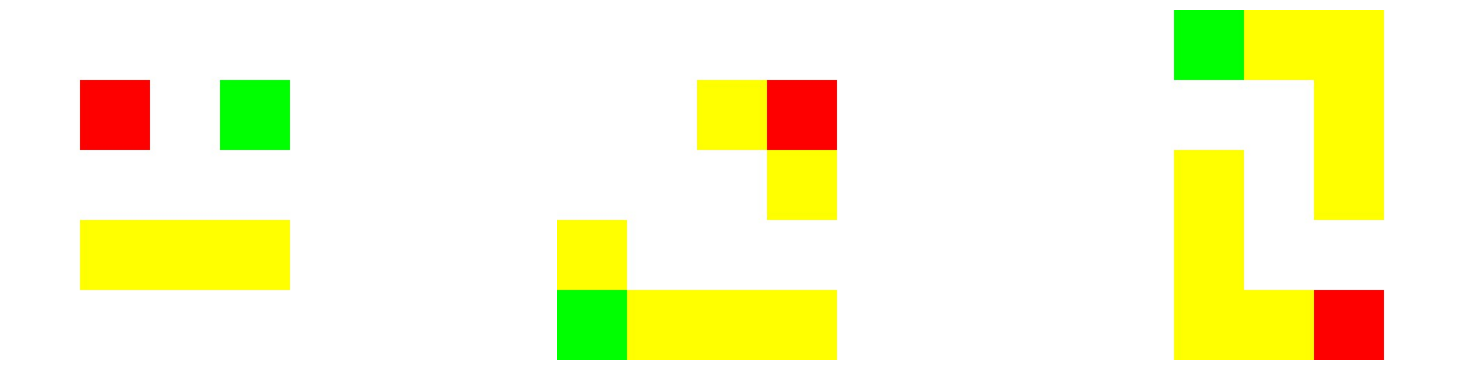
\includegraphics[width=\textwidth]{images/unsolvable_maze.png}
\caption{Examples of manually generated unsolvable mazes ($T=5$)}
\end{figure}

\newpage
\paragraph{Automatic}
For experimental purposes, the environment can also be constructed automatically using a greedy algorithm described below. 

\begin{algorithm}
    \caption{Greedy maze environment generation}\label{alg:cap}
    \begin{algorithmic}
        \Require $T \geq 2$
        \Ensure $|M| \geq 2, s \neq \emptyset, g \neq \emptyset$
        \State $L \gets \emptyset, M \gets \emptyset$
        \For{$x \gets 0, T$}
            \For{$y \gets 0, T$}
            \State $L \cup \{(x, y)\}$
            \EndFor
        \EndFor
        \State $s_M, g_M \gets$ randomSample$(L, 2)$
        \State $M \cup \{s_M, g_M\}$
        \State $c \gets s_M$
        \While{$c \neq g_M$}
            \State $c \gets$ randomSample$(L.$findNeighbours$(c), 1)$
            \If{$c \notin M$}
                \State $M \cup \{c\}$
            \EndIf
        \EndWhile
    \end{algorithmic}
\end{algorithm}
\noindent The algorithm begins by generating the set of all possible tile locations $L$. As expected, the size of $L$ is $T^2$. $M$ is a set of tiles that contains at least a path from the start tile $s_M$ to the goal tile $g_M$. In this form of generation, this is always the case, but $M$ may not have a path if it is created to be unsolvable through manual generation. The function randomSample$(a, b)$ returns $b$ randomly selected elements in array $a$ as an array of length $b$. If $b = 1$ then it returns the single element. This is used to randomly select a start and goal position, so that the algorithm can process a path between the two. In the processing of paths, a neighbour of the currently selected tile $c$, that is initially $s_M$ is added to $M$ until the neighbour of $c$ is $g_M$, which is the last tile that is added to $M$. Once a path is found, $M$ is defined by the set $\{c_0, ..., c_k\}$. This algorithm always ensures that $s_M$ is reachable from $g_M$ in $M$ as $c_0, ..., c_k$ is a path in $M$, where $c_0 = s_M$ and $c_k = g_M$, $k = |M|$. The average case time complexity of this algorithm is $O(T^2 + |M|)$, assuming that all operations are completed in linear time. In all cases, this does not affect the running time of the pipeline as the value of $T$ and $|M|$ are usually small enough ($\leq 100$) in comparison to the number of states evaluated during planning.
\begin{figure}[h!]
\centering
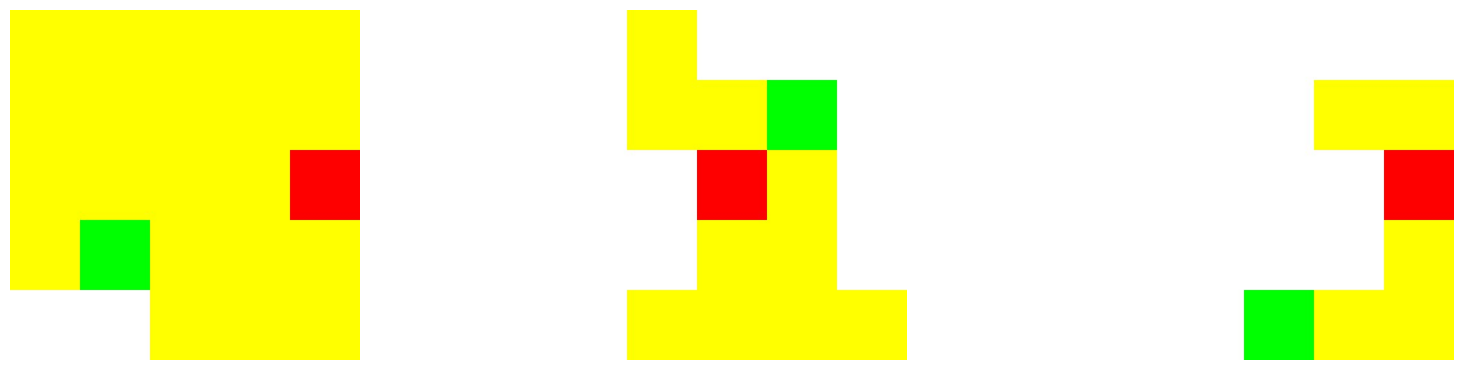
\includegraphics[width=\textwidth]{images/auto_maze_gen.png}
\caption{Examples of automatically generated mazes ($T=5$)}
\end{figure}

\newpage
\subsection{Domain}
The PDDL description of the Maze domain is shown in Figure 3.5 below.

\begin{figure}[h!]
$\text{Types} = \{position, direction\}\\\\
\text{Predicates} = \{Inc(a, b),\, Dec(a, b),\, At(x, y),\, Path(x, y),\, Facing(d),\, Is\mhyphen North(North),\,\\ Is\mhyphen East(East),\, Is\mhyphen South(South),\, Is\mhyphen West(West),\, Left\mhyphen Rot(d_n, d_{n-1}),\,\\ Right\mhyphen Rot(d_n, d_{n+1}))\}\\\\
\text{Actions} = \{\\
Action(move\mhyphen up(x, y, x_{new}, y_{new}, direction),\\
\text{\textsc{Precondition:}}\: Dec(y, y_{new}) \land At(x, y) \land At(x_{new}, y) \land Path(x_{new}, y_{new})\land Facing(direction) \land Is\mhyphen North(direction)\\
\text{\textsc{Effect:}}\: At(x_{new}, y_{new}) \land \neg At(x, y)),\\\\
Action(move\mhyphen down(x, y, x_{new}, y_{new}, direction),\\
\text{\textsc{Precondition:}}\: Inc(y, y_{new}) \land At(x, y) \land At(x_{new}, y) \land Path(x_{new}, y_{new})\land Facing(direction) \land Is\mhyphen South(direction)\\
\text{\textsc{Effect:}}\: At(x_{new}, y_{new}) \land \neg At(x, y)),\\\\
Action(move\mhyphen right(x, y, x_{new}, y_{new}, direction),\\
\text{\textsc{Precondition:}}\: Inc(x, x_{new}) \land At(x, y) \land At(x_{new}, y) \land Path(x_{new}, y_{new})\land Facing(direction) \land Is\mhyphen East(direction)\\
\text{\textsc{Effect:}}\: At(x_{new}, y_{new}) \land \neg At(x, y)),\\\\
Action(move\mhyphen left(x, y, x_{new}, y_{new}, direction),\\
\text{\textsc{Precondition:}}\: Dec(x, x_{new}) \land At(x, y) \land At(x_{new}, y) \land Path(x_{new}, y_{new})\land Facing(direction) \land Is\mhyphen West(direction)\\
\text{\textsc{Effect:}}\: At(x_{new}, y_{new}) \land \neg At(x, y)),\\\\
Action(turn\mhyphen left(direction, direction_{new}),\\
\text{\textsc{Precondition:}}\: Facing(direction) \land Left\mhyphen Rot(direction, direction_{new})\\
\text{\textsc{Effect:}}\: Facing(direction_{new}) \land \neg Facing(direction)),\\\\
Action(turn\mhyphen right(direction, direction_{new}),\\
\text{\textsc{Precondition:}}\: Facing(direction) \land Right\mhyphen Rot(direction, direction_{new})\\
\text{\textsc{Effect:}}\: Facing(direction_{new}) \land \neg Facing(direction))\}$\\
\caption{Blockly: Maze PDDL domain description}
\end{figure}

\newpage
\subsubsection{Defining the board}
All objects referring to the locations of tiles on a board have the type $position$. A position is the location of a tile on the maze. In this domain, an object with this type corresponds to a 1 dimensional coordinate. Predicates that involve a position take two position objects: an $x$ value and a $y$ value. Hence, instead of having $T^2$ positional objects, there are instead only $2T$ objects. $2T$ will always be less than $T^2$ as $T \geq 1$. The predicate $Inc(a, b)$ defines the locations in which the agent can move positively in the respective axis from position $a$ to $b$ by one unit. $a$ must be always greater than $b$, otherwise the agent facing $North$ could move in the $South$ direction. Similarly the predicate $Dec(a, b)$ ensures the agent can move negatively in the respective axis from position $a$ to $b$ by one unit, where $a \geq b$. Fluents with these predicates are only defined once and are never modified by any action.\\\\ The position of the agent is defined by the predicate $At(x, y)$. In all states, there can only be one fluent in which $At(x, y) = \top$ as the agent can only be in one location at any time. All problems in this domain have the initial state $I = At(s_{M_x}, s_{M_y})$ and goal state $G = At(g_{M_x}, g_{M_y})$. The locations that the agent can navigate is based on the truth value of the predicate $Path(x, y)$, where $(x, y) \in M$. Without defining $Inc$ and $Dec$, the agent could move from any two locations where $Path(x, y) = \top$, skipping sections of the maze, which is unintended. \\\\ In this domain, there are 4 objects with the $direction$ type: $North$, $East$, $South$ and $West$. The fluent $Facing(d) = \top$ states that the agent is currently facing direction $d$, this is verified by the predicates $Is\mhyphen North(North)$, $Is\mhyphen East(East)$, $Is\mhyphen South(South)$ and $Is\mhyphen West(West)$ which ensures that the input direction $d$ is truly the required direction. Similarly to $At$, the agent can only be facing one direction at any state. Finally, $Left\mhyphen Rot(d_n, d_{n-1})$ and $Right\mhyphen Rot(d_n, d_{n+1}))$ ensures that the new direction $d_{n\pm 1}$ is either left or right of $d$.

\subsubsection{Navigation}
The agent navigates the board by either moving or re-orientating. In each move action, given: the agent's current position $(x, y)$; a new position $(x_{new}, y_{new})$ and a $direction$. If there is a path to the new position, and the agent is facing the direction specified by $direction$, the agent will move to the new position and the fluent: $At(x, y)$ is set to $\bot$ as the agent is no longer in that location. In the case of the action $move\mhyphen up$, the agent must be facing $North$, and there must be a decrement between the two given $y$ position objects, as the $North$ direction in the domain is $-y$ in the real world. The actions $move\mhyphen down$, $move\mhyphen right$ and $move\mhyphen left$ performs the same action in their respective directions. The decision to not conflate these actions into a single move action was due to the planner support for disjunctive preconditions. Determining the direction to move in, given the direction would involve evaluating the statement: 
\begin{align*}
    &(Is\mhyphen North(North) \land Dec(y, y_{new}) \land At (x_{new}, y))\\
    &\lor (Is\mhyphen South(South) \land Inc(y, y_{new}) \land At(x_{new}, y))\\
    &\lor ...
\end{align*}
For each turning action, given the current $direction$ and a new direction, $direction_{new}$, if the agent is facing the current direction and, in the case of $move\mhyphen left$, there is a left rotation possible from $direction$ to $direction_{new}$, the agent is will now face the direction $direction_{new}$ and no longer be facing $direction$. Similarly $move\mhyphen right$ causes the agent face $direction_{new}$ if there is a right rotation possible from $direction$ to $direction_{new}$.

\subsection{Problem Generation}

\subsubsection{Objects}
As mentioned in the previous section, there are $2T$ positional objects in this domain defined by: $X_M = \{x_0, x_2, ..., x_{T-1}\}$ and $Y_M = \{y_0, y_2, ..., y_{T-1}\}$. The top-left tile position is object tuple: $(x_0, y_0)$. The direction objects for all problems in this domain is given by the set $D = \{North, East, South, West\}$.

\subsubsection{Initial State}
The initial state $I$ is given by the conjunction of the following fluents. The below table (Table 3.1) shows the fluents along with a description explaining what it refers to in the Maze.

\begin{table}[ht]
\centering
\begin{tabular}{|p{0.473\linewidth}|p{0.473\linewidth}|}
\hline
Fluents & Description \\\hline
$\forall x \in X_M, Inc(x_n, x_{n+1}) = \top$. $\forall y \in Y_M, Inc(y_n, y_{n+1}) = \top$.& For every position object in $X_M$, $x_{n}$ neighbours the object $x_{n+1}$ where $x_{n+1}$ is $North$ of $x_n$. Similarly for every position object in $Y_M$, where the neighbour is $East$. \\\hline
$\forall x \in X_M, Dec(x_n, x_{n+1}) = \top$. $\forall y \in Y_M, Dec(y_n, y_{n+1}) = \top$.& For every position object in $X_M$, $x_n$ neighbours the object $x_{n-1}$ where $x_{n-1}$ is $South$ of $x_n$. Similarly for every position object in $Y_M$, where the neighbour is $West$. \\\hline
$\forall t \in M, Path($toObj$(t_x)$, toObj$(t_y)) = \top$& For all tiles in the Maze $M$, the agent can traverse the position $(t_x, t_y)$.\\ \hline
$\forall d \in D, Is\mhyphen d(d) = \top$& In all directions, the direction object $d$ is truly the position specified by $d$. I.e if $d = North$, then $Is\mhyphen North(North) = \top$~ \\\hline
$\forall d \in D, Right\mhyphen rot(d, d_{n+1}) = \top$. $\forall d \in D, Left \mhyphen rot(d, d_{n-1}) = \top$& In all directions, there is a right rotation from the object $d$ to the object right of it, $d_{n+1}$. Similarly there is a left rotation from the object $d$ to the object left of it, $d_{n-1}$. \\\hline
$facing(North) = \top$& The agent is always initially facing $North$ \\\hline
$at(toObj(s_{M_x}), toObj(s_{M_y})) = \top$& As mentioned in the previous section, the start location is set by this fluent. \\\hline
\end{tabular}
\caption{Initial state $I$ in the Maze domain}
\end{table}
\noindent All other state variables not included here are set to $\bot$.

\subsubsection{Goal}
The goal is for the agent to be at tile location $g_M$: $G = At($toObj$(g_{M_x}), $toObj$(g_{M_y}))$

\newpage
\subsubsection{Example Plan}
Problem 9 in Blockly Games: Maze can be solved in a plan with 26 lines using Fast Downward:

\begin{figure}[h!]
\centering
\begin{BVerbatim}
0: turn-right(north, east)
1: move-right(x12, y16, x13, y16, east)
2: move-right(x13, y16, x14, y16, east)
3: turn-left(east, north)
4: move-up(x14, y16, x14, y15, north)
...
11: move-up(x14, y9, x14, y8, north)
12: turn-left(north, west)
13: move-left(x14, y8, x13, y8, west)
...
25: move-left(x2, y8, x1, y8, west)
\end{BVerbatim}
\caption{Solution to Problem 9 of Maze using the Blockly-Maze Problem Generator}
\end{figure}



\section{Problem Reduction on the Board}
% Talk about necessity for this reduction
As shown in the Experiments section, the generalised planner does not perform well on the initial Maze problems, taking up lots of memory even for the most basic of problems. To scale the size of the problems, I performed a problem reduction. This involved flattening the number of actions to just a single move action and removing predicates involving direction. The direction is instead implied through the use of naming objects or by observing the positions used in move actions. This leads to a significant performance increase as shown in the results, however there is a large loss in information, and takes away from the Blockly setting. The complexity behind the problems instead comes from its generation rather than its solution, making it significantly easier for the planner yet harder on the interpreter which nonetheless, could compute the instructions faster.

\subsection{Revised Domain}
The revised PDDL description of the Maze domain after performing a grid based problem reduction is shown in Figure 3.6 below.

\begin{figure}[h!] 
$\text{Types} = \{position, direction\}\\\\
\text{Predicates} = \{At(x), Path(x, y)\}\\\\
\text{Actions} = \{\\
Action(move(x, x_{new}),\\
\text{\textsc{Precondition}}:\: At(x) \land Path(x, x_{new})\\
\text{\textsc{Effect}}:\: At(x_{new}) \land \neg At(x))\}\\$
\caption{Problem reduced Maze PDDL domain description}
\end{figure}

\subsubsection{Re-defining the Board}
Objects with the $position$ type now correspond to 2 dimensional coordinates containing values for both $x$ and $y$. The predicate $At(x)$ retains its original meaning, whereas $Path(x, y)$ now states that the agent can move from position $x$ to position $y$ instead of stating that the defined position can be traversed. 

\subsubsection{Faster Navigation}
The agent now navigates the board through moving only. When the agent moves, its orientation is already implied from the initial and destination locations. As long as the agent can move from $x$ to $x_{new}$, then it will make that move. The new domain reduces the number of actions considered between moving from state to state leading to faster navigation speeds.

\subsection{Directional Problem Generation}
The allocation of objects to tiles is given by the set of mappings $R$. Each element of $R$ contains a mapping with syntax map$(O \rightarrow t)$, where $O$ is a PDDL object and $t$ is the tile position. There is a one-to-many relationship from object to tile positions, where each position can have up to four objects: $up$, $down$, $left$ and $right$. The object $O$ that maps to $t$ is determined from the direction of travel from one of $t$'s neighbours to $t$, an example illustration is given below in Figure 3.7.

\begin{figure}[h!]
    \ctikzfig{images/directionaldemo}
    \caption{Directional object generation example}
\end{figure}

\noindent To ensure no object names are repeated, there is a counter $i$ that increments after a tile has been visited. In this example the object \texttt{r6} is the goal position. The algorithm always visits the directions in following order: $u_i (up)$, $d_i (down)$, $l_i (left)$ and finally $r_i (right)$. Each tile has a is the set of tile neighbourhood mappings $D$ where $D_j =$ map$(d_D \rightarrow n_D)$ is the mapping at index $j$. $d_D$ is the PDDL object of a direction and $n_D$ is the tile position of the neighbour in the direction of $d_D$, in the mapping of $D_j$. With this, the orientation of the agent can easily be inferred, however there comes with the drawback of having more than four times as many objects in the worst case scenario than in the original Maze definition. Overall, in this domain, there are at most $R \leq 4 \times |M|$ objects. The full algorithm that generates these objects as well as the paths between them is defined below in Algorithm 2.

\newpage
\begin{algorithm}[h!]
    \caption{Directional object generation and path setting}\label{alg:cap}
    \begin{algorithmic}
        \Require $|M| \geq 2, s_M \neq \emptyset, g_M \neq \emptyset,$ a path $p$: $c_0, ..., c_k$ 
        in the graph of $M$ where $c_0 = s_M, c_k = g_M$
        \Ensure $|R| \geq |p|$
        \State $i \gets 0$
        \State $R = \emptyset$
        \Procedure{DFSOG}{mapping $m$}
            \State $R \cup \{m\}$
            \State map$(O \rightarrow t) \gets m$
            \State $D \gets$ mapping of objects in $\{u_i, d_i, r_i, l_i\}$ to the neighbours of $t$
            % \{("up_i" \rightarrow (t_x, t_y - 1)), ("down_i" \rightarrow (t_x, t_y + 1)), ("left_i" \rightarrow (t_x - 1, t_y)), ("right_i" \rightarrow (t_x + 1, t_y))\}$
            \For{$j \gets 0, (|D| - 1)$}
                \State map$(d_D \rightarrow n_D) \gets D_j$
                \If{$n \in M$}
                    \For{$k \gets 0, (|R| - 1)$}
                    \State map$(d_R \rightarrow n_R) \gets R_k$
                    \If{$d_D = d_R$}
                        \State $I \gets I \cup \langle Path(O, d_R) = \top \rangle$ \Comment{Create paths to existing objects}
                        \State skip to next $j$
                    \EndIf
                    \EndFor
                \EndIf
                \If{$n_D = s_M$}
                    \State $D_j \gets $map$($toObj$(s) \rightarrow n_D)$
                \EndIf
                \If{$n_D = g_M$}
                    \State $D_j \gets $map$($toObj$(g) \rightarrow n_D)$
                \EndIf
                \State $I \gets I \cup \langle Path(O, d_D) = \top \rangle$
                \State $i \gets i + 1$
                \State \Call{DFSOG}{$D_j$}
            \EndFor
        \EndProcedure
        \State \Call{DFSOG}{$($map$($toObj$(s_M) \rightarrow s_M)$}
    \end{algorithmic}
\end{algorithm}

\noindent To clarify, the notation $I \gets I \cup \langle F \rangle$ adds the fluent $F$ to the initial state $I$. This algorithm computes a depth first search \cite{depthfirstsearch} over the set of tiles used in the Maze $M$. In the graph of $M \rightarrow G_M(V, E)$, the set of tiles are the vertices $V$, and each vertex $c$ has an edge to each of its neighbours, such that for each neighbour $v \in M$.findNeighbours$(c)$, $(c, v)$ is an edge in $E$. Therefore if there is a vertex $c_0 = s_M$ and a vertex $c_k = g_M$ in G, and the starting position is reachable from the goal position in $M$, then there is a path $p$: $c_0, ..., c_k$. Usually, this is always the case as the automatic generation algorithm is used to generate Mazes in experiments, which generates a path in $G_M$

\subsubsection{Start and Goal}
Similarly to the initial Maze domain, the start position of the agent is given by setting the fluent: $At($toObj$(s_M)) = \top$, and the goal is for the planner to set the fluent $At($toObj$(g_M)) = \top$.

\newpage
\subsubsection{Example Plan}
Problem 9 in Blockly Games: Maze can be solved in a plan with 22 lines using Fast Downward:\\
\begin{figure}[h!]
\centering
\begin{BVerbatim}
0: move(start, r0)
1: move(r0, r1)
2: move(r1, u2)
3: move(u2, u3)
4: move(u3, u4)
...
17: move(l32, l33)
18: move(l33, l40)
19: move(l40, l41)
20: move(l41, l44)
21: move(l44, goal)
\end{BVerbatim}
\caption{Solution to Problem 9 of Maze using the Directional Problem Generator}
\end{figure}

\subsection{Non-Directional Problem Generation}
Due to the large number of objects generated by the above directional problem generator, this generator focuses solely on simple path planning problems. There are $|M|$ objects in each problem where each object corresponds to an $(x, y)$ coordinate. The naming scheme for an object, given a tile $t$ is: \texttt{p}$t_x$\texttt{-}$t_y$. In the best case scenario, problems of this kind can be solved four times as fast as the previous generator. In the worst case, it will perform equally as good. As this report focuses on the synthesis of plans involving complex path planning problems, this will not be included in the evaluation of such. However this is necessary to include, as it acts as the foundation for the Snake problem generator.

\subsubsection{Example Plan}
Problem 9 in Blockly Games: Maze can be solved in a plan with 20 lines using Fast Downward:

\begin{figure}[h!]
\centering
\begin{BVerbatim}
0: move(p13-12, p14-12)
1: move(p14-12, p14-11)
2: move(p14-11, p14-10)
3: move(p14-10, p14-9)
4: move(p14-9, p14-8)
...
15: move(p6-6, p5-6)
16: move(p5-6, p4-6)
17: move(p4-6, p3-6)
18: move(p3-6, p2-6)
19: move(p2-6, p1-6)
\end{BVerbatim}
\caption{Solution to Problem 9 of Maze using the Non-Directional Problem Generator}
\end{figure}

\newpage
\section{Snake Problem Generation}
A Snake environment consists of four main components:

\begin{itemize}
    \item \textbf{Board}: A collection of tile objects $B$ representing the available locations for the snake to traverse. The size of the board is always fixed at size $T^2$.
    \item \textbf{Head}: The initial location of the snake's head $h_B$, there can only be one starting location per maze environment
    \item  \textbf{Tail}: The initial location of snake's tail $t_B$, indicating the initial blocked tile on the board.
    \item \textbf{Apples}: The tile locations of apples on the grid $A_B$
\end{itemize}

\subsection{Generation}
The environment is always constructed through automatic generation, by first creating all the tiles on the board, followed by the start and apples. The red tile, represents the position of the head of the snake and the blue tile represents the position of the tail. When an apple is added to the board, the consequent apple is darkened, indicating that the apple is collected subsequently. The locations of these apples are chosen randomly and never appear on top of each other or on the start positions, hence a limit on the number of apples is $T^2 - 2$. Another limit on the number of apples is 255, due to the 8-bit colour depth thats factored in when creating the variations of green in the Pygame display.

\begin{figure}[h!]
\centering
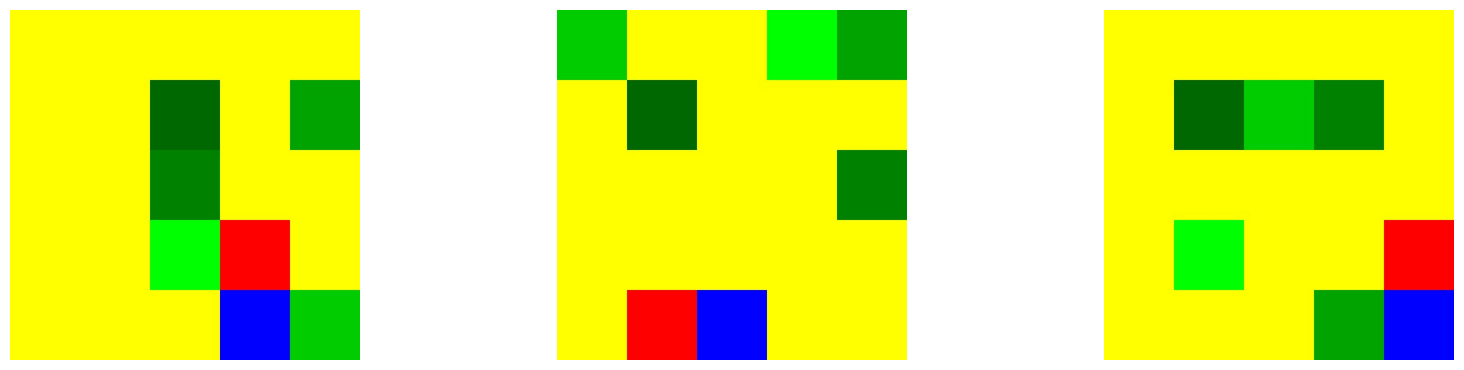
\includegraphics[width=\textwidth]{images/snake5x5autogen.png}
\caption{Examples of Snake environments ($T=5, |A_B|=5$).}
\end{figure}

\begin{figure}[h!]
\centering
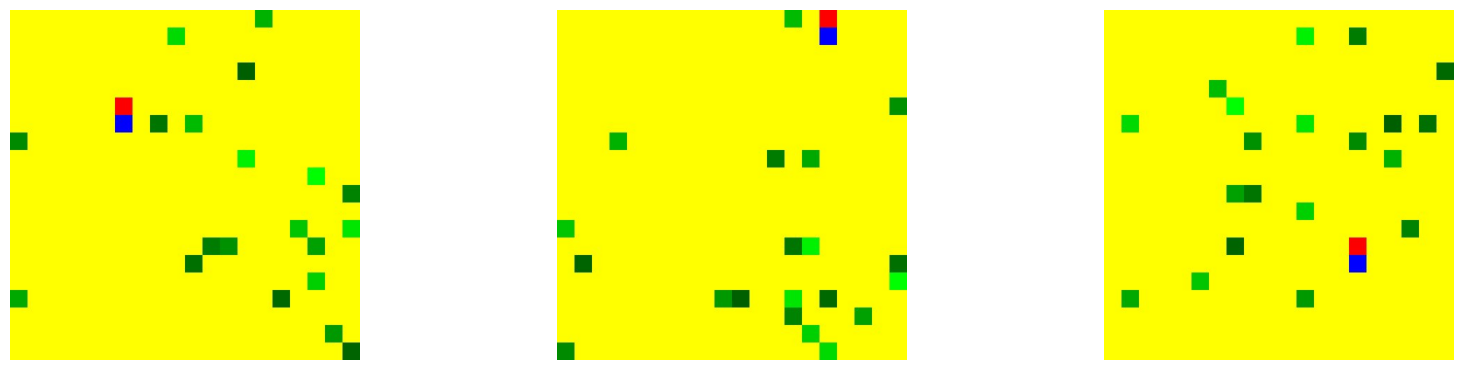
\includegraphics[width=\textwidth]{images/snake20x20autogen.png}
\caption{Examples of larger Snake environments ($T=20, |A_B|=20$).}
\end{figure}

\newpage
\subsection{Domain}
The positioning system used in this domain is the same as the one used in the Non-Directional Maze domain, to obtain the best possible results when solving problems. This domain is an adaptation of the IPC 2018's Optimal Snake, where constants have been removed to make it suitable for the generalised planner to generate plans from problems in this domain. Below in Figure 3.10 is the full definition of this domain.

\begin{figure}[h!] 
$\text{Types} = \{position\}$ \\\\
$\text{Predicates} = \{Path(x, y), Head\mhyphen At(x), Tail\mhyphen At(x), Body\mhyphen Con(x), Blocked(x),\\Apple\mhyphen at(x), Spawn\mhyphen apple(x), Next\mhyphen Apple(x, y), Is\mhyphen DummyPoint(x)\}\\\\
\text{Actions} = \{\\
Action(move(head, head_{new}, tail, tail_{new}),\\
\text{\textsc{Precondition:}}\: Head\mhyphen At(head) \land Path(head, head_{new}) \land Tail\mhyphen At(tail) \land Body\mhyphen Con(tail_{new}, tail) \land \neg Blocked(head_{new}) \land \neg Apple\mhyphen At(head_{new})\\
\text{\textsc{Effect:}}\: Blocked(head_{new}) \land Head\mhyphen At(head_{new}) \land Tail\mhyphen At(tail_{new}) \land Body\mhyphen Con(head_{new}, head)) \land \neg Head\mhyphen At(head) \land \neg Blocked(tail) \land \neg Tail\mhyphen At(tail) \land \neg Body\mhyphen Con(tail_{new}, tail)),\\\\
Action(move\mhyphen and\mhyphen eat(head, head_{new}, spawn, spawn_{next}),\\
\text{\textsc{Precondition:}}\: Head\mhyphen At(head) \land Path(head, head_{new}) \land Apple\mhyphen At(head_{new}) \land Spawn\mhyphen Apple(spawn) \land Next\mhyphen Apple(spawn, spawn_{next}) \land \neg Blocked(head_{new}) \land \neg Is\mhyphen DummyPoint(spawn)\\
\text{\textsc{Effect:}}\: Blocked(head_{new}) \land Head\mhyphen At(head_{new}) \land Apple\mhyphen At(spawn) \land Spawn\mhyphen Apple(spawn_{next})) \land \neg Head\mhyphen At(head) \land \neg Apple\mhyphen At(head_{new}) \land \neg Spawn\mhyphen Apple(spawn)),\\\\
Action(move\mhyphen and\mhyphen eat\mhyphen no\mhyphen spawn(head, head_{new}, dummypoint),\\
\text{\textsc{Precondition:}}\: Head\mhyphen At(head) \land Path(head, head_{new}) \land Apple\mhyphen At(head_{new}) \land Spawn\mhyphen Apple(dummypoint) \land Is\mhyphen DummyPoint(dummypoint) \land \neg Blocked(head_{new})\\
\text{\textsc{Effect:}}\: Blocked(head_{new}) \land Head\mhyphen At(head_{new}) Body\mhyphen Con(head_{new}, head)\\ \land \neg Head\mhyphen At(head) \land \neg Apple\mhyphen At(head_{new})\}$

\caption{Snake PDDL domain description}
\end{figure}

\subsubsection{Defining the Snake board}
This domain follows the same positioning system as mentioned in the Non-directional problem generator. Each object with the $position$ type corresponds to a 2 dimensional coordinate. Similarly, the fluent $Path(x, y) = \top$ states that the Snake can move from position $x$ to position $y$. A position $x$ is unusable, regardless if there is a path if $Blocked(x) = \top$. A path is blocked if any part of the Snake is occupying it. The fluent $Apple\mhyphen At(x)$ states that there is an apple that can be collected by the Snake at position $x$. 

\subsubsection{Getting Around}
When the Snake moves, the tail always follows the head. The fluent $Head\mhyphen At(x) = \top$ states that the head is position $x$. $Tail\mhyphen At(x) = \top$ is the same, but for the tail. The tiles occupied between the head and the tail are given by $Body\mhyphen Con(x)$ where $x$ is a position that belongs to the snake's body. The action 
$move$ moves the head position by one unit to $head_{new}$ and blocks that position, so that the snake cannot go back in on itself. The tail position is moved to $tail_{new}$ where $tail_{new}$ must be a part that is connected to the body of the snake, and the original tail position $tail$ is unblocked as the Snake no longer occupies it. The illustration below in Figure 3.11 shows this process.

\begin{figure}[h!]
    \ctikzfig{images/snakemovedemo}
    \caption{Snake of length 3, with the head moving left.}
\end{figure}


\subsubsection{Collecting Apples}
When the snake moves on to a location containing an apple, the Snake eats it and grows in size. To simulate this effect, the head moves without the tail, increasing the gap between the positions. The next apple is then spawned at the location $x$ given in $Spawn\mhyphen Apple(x)$. After an apple is spawned the next spawn location $y$ is given in $Next\mhyphen Apple(x, y)$. This is then updated until there are no more defined spawnable locations in the problem. After all apples are collected by the Snake, a $dummypoint$ is placed on an arbitrary location that does not belong to the board. This is so the spawn sequence induced by $Next\mhyphen Apple$, terminates. This is done in the $move\mhyphen and\mhyphen eat\mhyphen no\mhyphen spawn$ action, where the future spawn location must be the $dummypoint$ checked by the predicate $Is\mhyphen DummyPoint$. There is only a single chain of apples being generated during the problem generation, hence this action will only be used once at the end of the plan.

\subsection{Problem Generation}
\subsubsection{Objects}
The set of objects, which are all positions, is given by $X_B = \{x_1, ..., x_{|B|}\} \cup \{dummypoint\}$, where $x$ corresponds to a unique position in $B$. The set of apples $A_B$ contains a random location not on the board as its last element, in which calling the function toObj on it references $dummypoint$.

\subsubsection{Initial State}
Similar to the table in the Maze section, the below table (Table 3.2) shows the fluents set to $\top$ that form part of the initial state $I$ in problems with this domain.

\begin{table}[ht]
\centering
\begin{tabular}{|p{0.473\linewidth}|p{0.473\linewidth}|}
\hline
Fluents & Description \\\hline
$\forall x \in X_B, Path(x, x_{n + 1}) = \top$. & For every position object in $X_B$, $x_{n}$ neighbours the object $x_{n+1}$ where $x_{n+1} \in B.$getNeighbours$(t)$ where $t$ is the tile position represented by the object $x$. \\\hline
$Head\mhyphen At($toObj($h_B)) = \top$. & The head is initially at the position $h_B$. $h_B \neq t_B,\, h_B \notin A_B$. \\\hline
$Tail\mhyphen At($toObj($t_B)) = \top$. & The tail is initially at the position $t_B$. $t_B \neq h_B,\, t_B \notin A_B$. \\\hline
$Body\mhyphen Con($toObj($h_B), $toObj($t_B)) = \top$ & The body is initially connected only to the head and the tail. The Snake has an initial length of 2. \\\hline
$Blocked($toObj($h_B)) = \top$\hfill, $Blocked($toObj($t_B)) = \top$ & Intially, the head and tail positions are inaccessible, as it belongs to the body of the Snake.\\\hline
$\forall a \in A_B, Apple\mhyphen At($toObj$(a)) = \top$& This defines the initial locations of all apples. \\\hline
$Spawn\mhyphen Apple($toObj$(a_1)) = \top$& $a_1$ is the first apple spawned after $a_0$ has been eaten. \\\hline
$\forall a \in A_B \setminus \{a_0\}$\hfill, $Next\mhyphen Apple($toObj$(a), $toObj$(a_{n+1})) = \top$& The next apple to spawn after $a$ has been spawned is $a_{n+1}$ for each apple in $A_B$.  \\\hline
$Is\mhyphen DummyPoint(dummypoint) = \top$& The object $dummypoint$ is truly the $dummypoint$.  \\\hline
\end{tabular}
\caption{Initial state $I$ in the Snake domain}
\end{table}

\subsubsection{Goal}
The goal $G$ in this domain is given by: $G = \{Apple\mhyphen At(a) = \bot \mid a \in A_B\}$, which states that all apples, set in the problem, must be eaten by the Snake.

\newpage 
\section{Compilation and Generating Plans}
After $\mathcal{P}$ has been defined through generating classical planning instances $P$ using the problem generators, it is then built into a Unified Planning problem using Python. An example of a problem generated using the Directional problem generator is given in the Appendix. After the problem has been created, it can be solved using classical planning, in which each $P \in \mathcal{P}$ is solved individually, or through generalised planning where $\mathcal{P}$ is evaluated all at once. This process can be done using two methods:

\subsection{Generating Plans using the Command Line Interface (CLI)}
Plans can be generated through the use of a CLI. The user can choose to generate problems from the selection of generators: \texttt{blockly\_maze}, \texttt{directional\_maze}, \texttt{non\_directional\_maze} and \texttt{snake}. An example command that generates a single problem using automatic generation, where $T=5$ and classical planning is used in the Maze domain, is given in Figure 3.15 below:

\begin{figure}[h!]
    \centering
    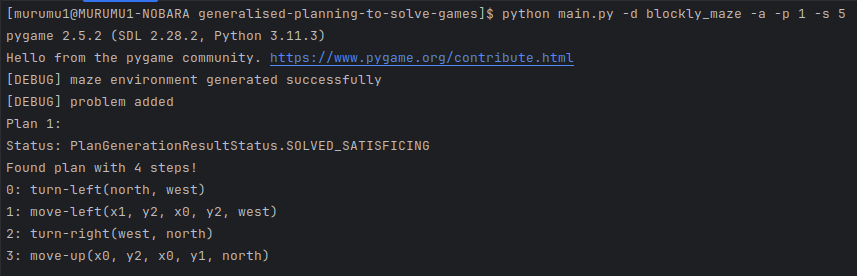
\includegraphics[width=\textwidth]{images/terminalexample.png}
    \caption{Example CLI usage}
\end{figure}

\noindent A full description of all flags is given in the Appendix.

\subsection{Generating Plans using a Jupyter Notebook}
This project can be imported as a library to produce visuals that can be used within a Jupyter Notebook. Each generator is thoroughly documented and can be extended to provide more functionality. Furthermore, developers can make use of the \texttt{ProblemGenerator} class to create more instances of path finding problems. There are five functions that can be used on any generator:

\begin{itemize}
    \item \texttt{save\_as\_pddl()} saves all problems as individual PDDL problem files to a folder set by \texttt{problem\_directory}.
    \item \texttt{display\_problems()} displays all problems written as Unified Planning problem instances.
    \item \texttt{display\_images(columns=None)} displays all problems as images as plots that can only be generated within Jupyter Notebook. The \texttt{columns} parameter determines how many images to fit on a single row in the output.
    \item \texttt{solve\_each()} solves all problems individually using Fast Downward
    \item \texttt{solve\_all(program\_lines=10)} solves all problems at once using BFGP++.
\end{itemize}
\noindent Below in Figure 3.16 is an example of generating a set of 10 plans, with images that represent the problems:

\begin{figure}[h!]
    \centering
    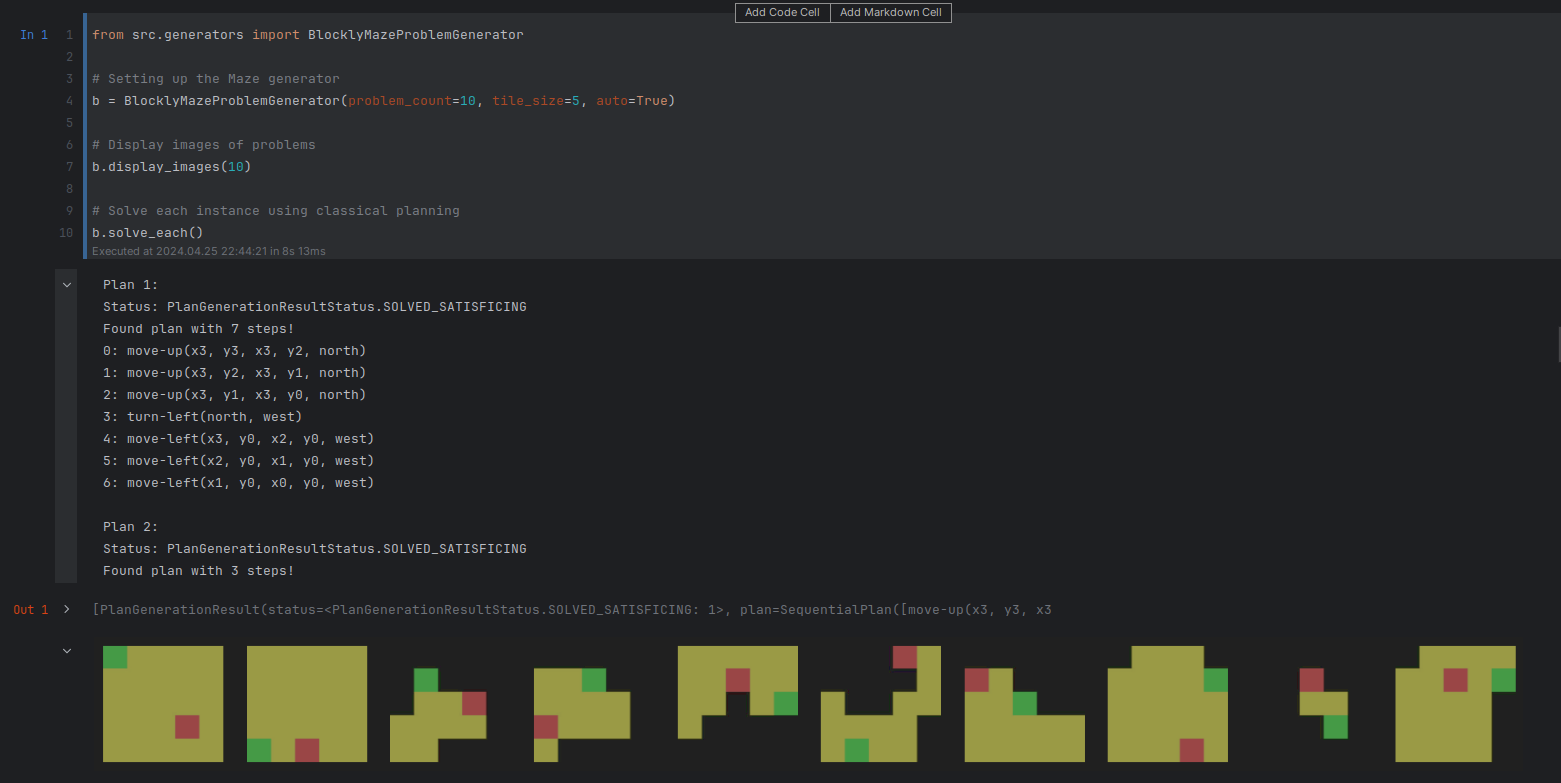
\includegraphics[width=\textwidth]{images/jupyternotebook.png}
    \caption{Example Jupyter Notebook usage}
\end{figure}

\subsection{Obtaining Classical Plans from a Generalised Plan}
After a generalised plan has been synthesised, a folder set by \texttt{plan\_directory} is generated that contains the classical plans generated by the generalised plan. In the case of the following problems:

\begin{figure}[h!]
    \centering
    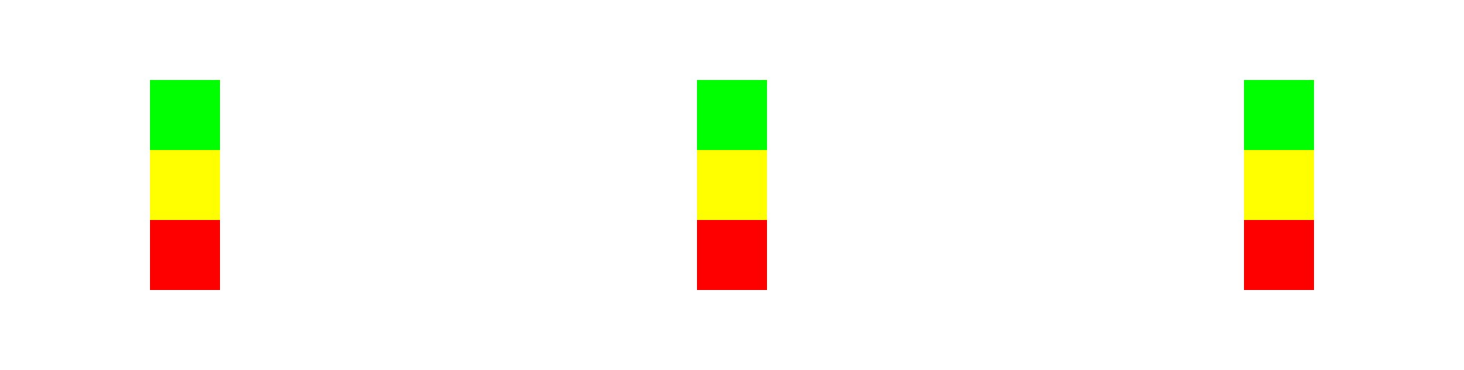
\includegraphics[width=\textwidth]{images/similargenplanning.png}
    \caption{Example problems used in a generalised planning demonstration}
\end{figure}

\newpage
\noindent The \texttt{.prog} file contains the generalised solution in 10 lines:

\begin{figure}[h!]
    \centering
    \begin{BVerbatim}
0. for(ptr_position_0++,8)
1. for(ptr_position_1++,3)
2. move(ptr_position_0,ptr_position_1)
3. endfor(ptr_position_1++,1)
4. for(ptr_position_1--,7)
5. move(ptr_position_1,ptr_position_0)
6. move(ptr_position_0,ptr_position_1)
7. endfor(ptr_position_1--,4)
8. endfor(ptr_position_0++,0)
9. end
    \end{BVerbatim}
\end{figure}

\noindent Which generates the following solution in \texttt{plan.}$k$, where $1 \leq k \leq |\mathcal{P}|$. In this case, the plan is the same in all \texttt{plan} files as they are the same problem:

\begin{figure}[h!]
\centering
\begin{BVerbatim}
(move start_ u0)
(move u0 start_)
(move start_ u0)
(move u0 goal_)
(move goal_ d2)
(move d2 goal_)
\end{BVerbatim}
\caption{Inefficient solution generated by a generalised plan}
\end{figure}